% Gerado por experimentos/conteudo/graficos.py. Requer \usepackage{graphicx}.
\begin{figure*}[htbp]
\centering
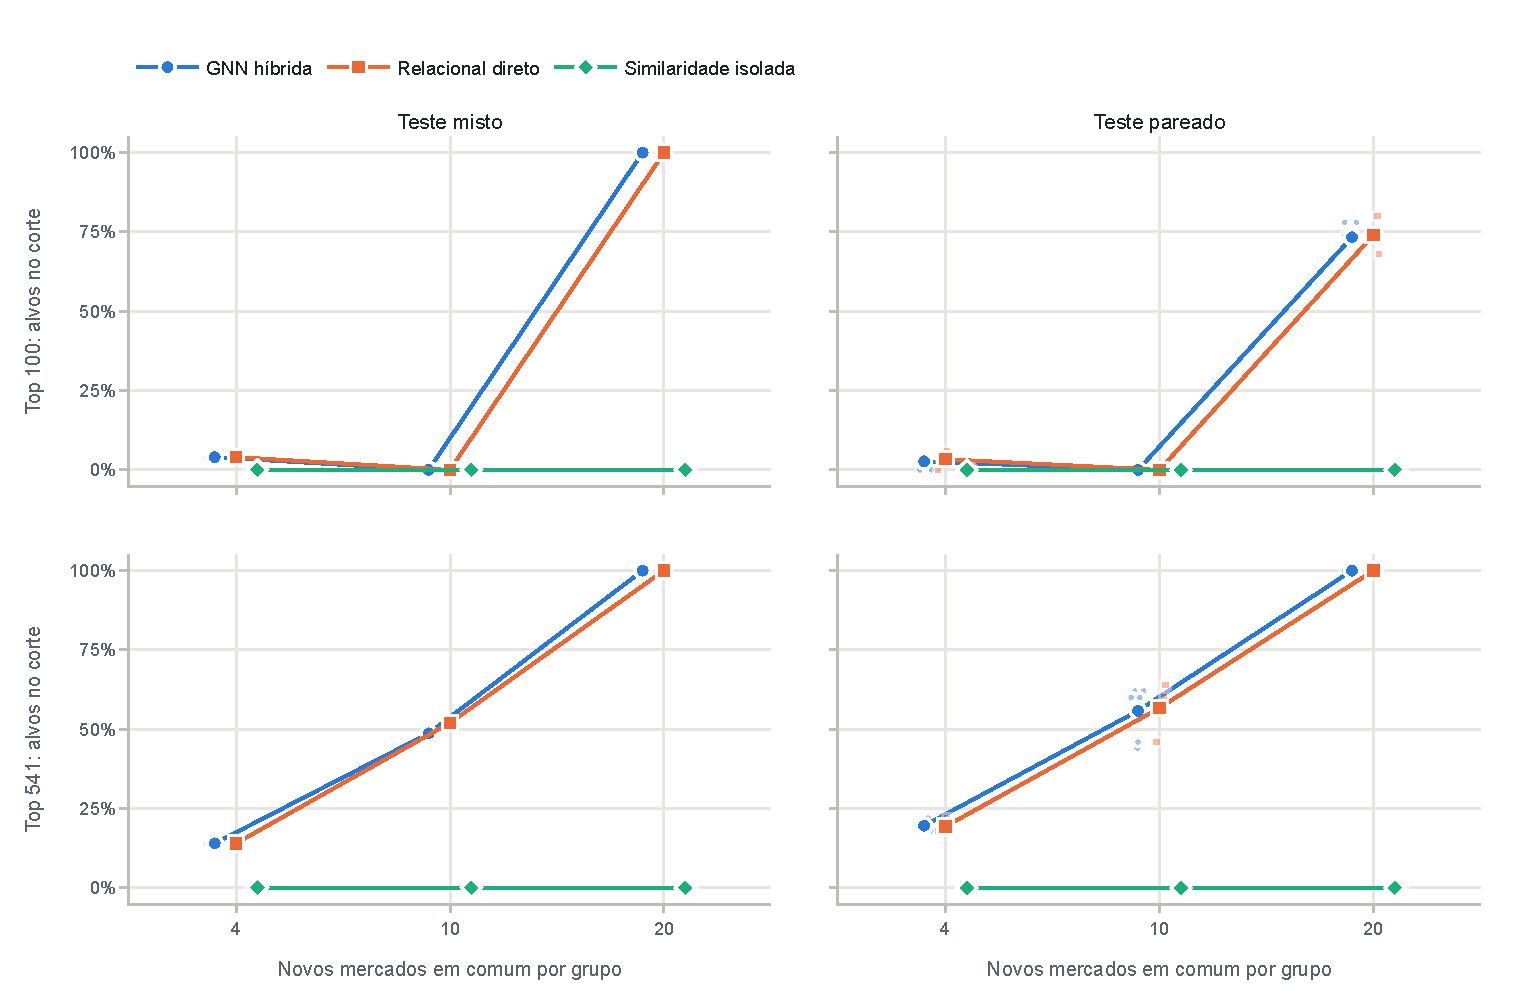
\includegraphics[width=\textwidth]{G1_recuperacao_intensidade.pdf}
\caption{Recuperação dos alvos artificiais por intensidade. Percentual dos 50 alvos no top 100 (acima) e no top 541 (abaixo). Pontos claros: cada ranking (misto: soma dos três sorteios por seed; pareado: cada sorteio e seed); marcadores ligados: média. O relacional é determinístico (um ranking por sorteio). Mesma escala nos quatro painéis.}
\label{fig:g1}
\end{figure*}

\begin{figure}[htbp]
\centering
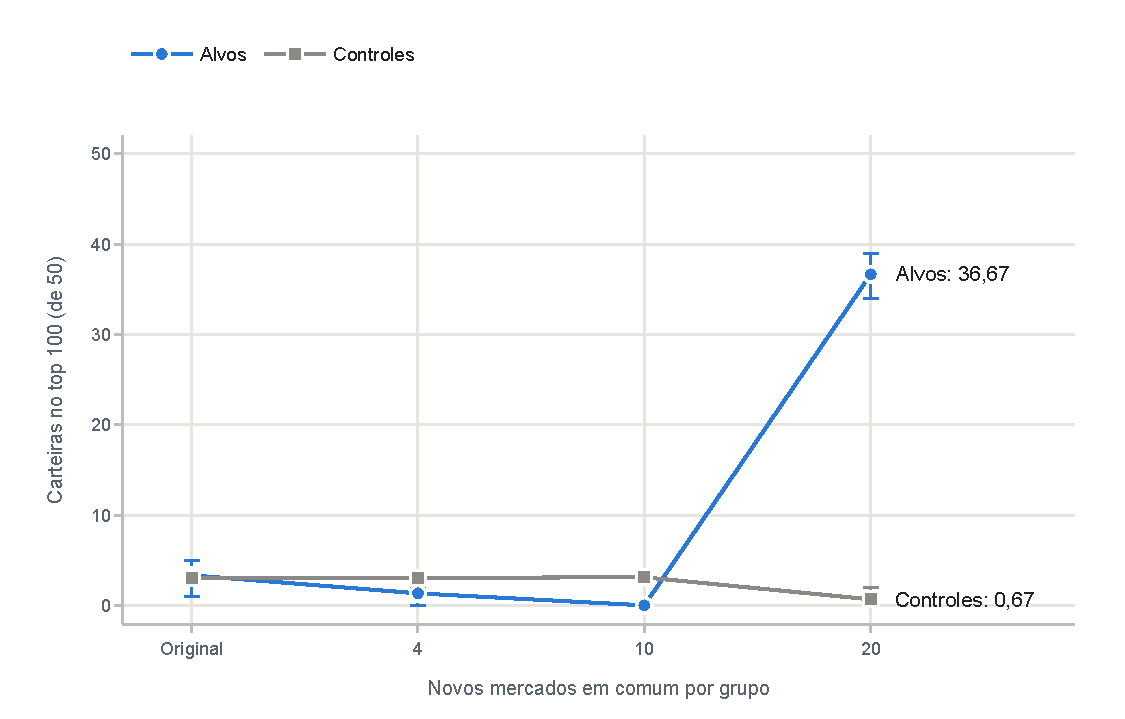
\includegraphics[width=\columnwidth]{G2_alvos_vs_controles.pdf}
\caption{Alvos e controles no teste pareado (GNN híbrida). Média de carteiras no top 100, de 50 em cada categoria. Unidade: sorteio (média das três seeds); as barras vão do menor ao maior dos três sorteios. Controles têm o mesmo grau inicial do alvo e ligações intactas.}
\label{fig:g2}
\end{figure}

\begin{figure*}[htbp]
\centering
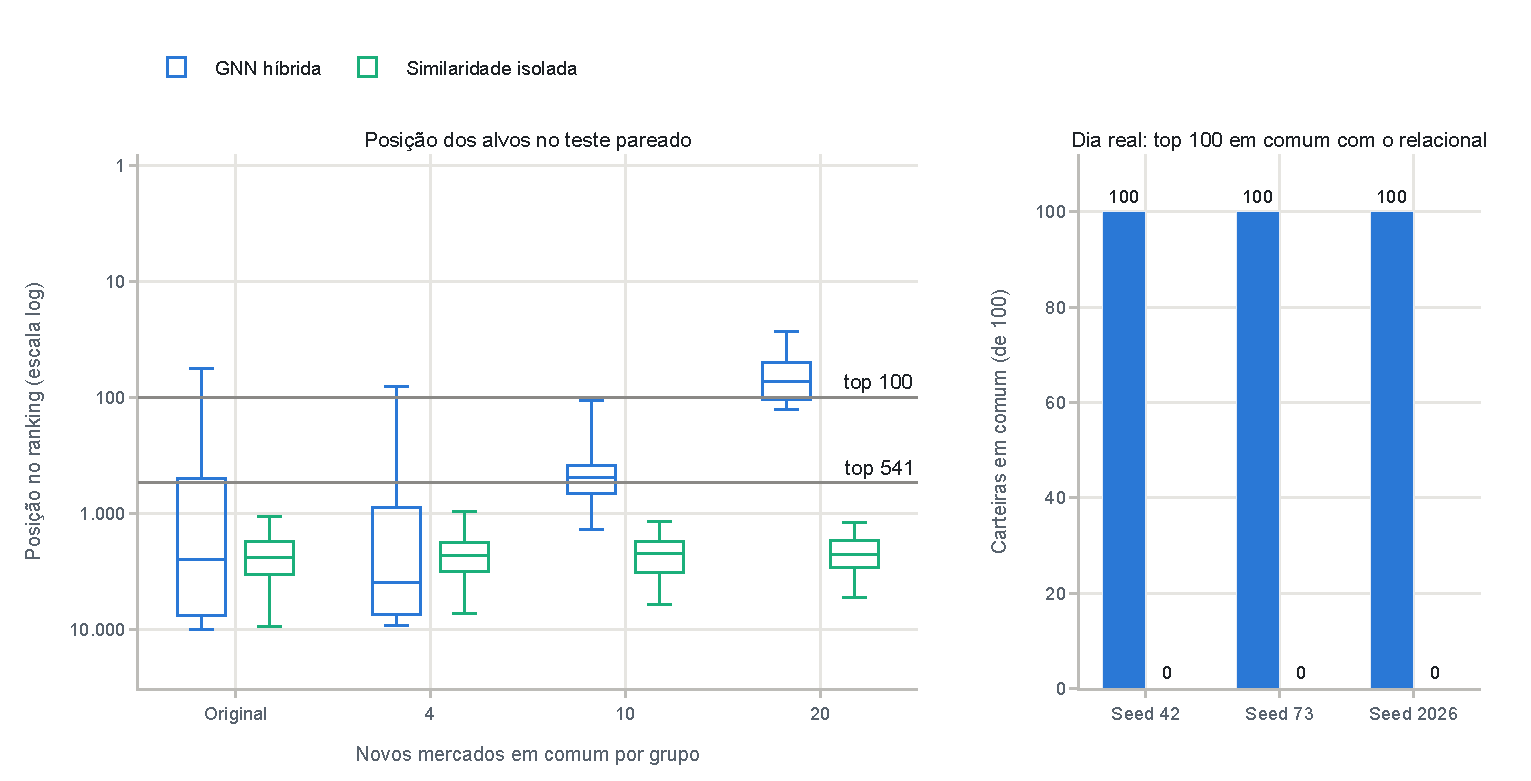
\includegraphics[width=\textwidth]{G4_comparacao_gnns.pdf}
\caption{GNN híbrida versus similaridade isolada. As duas usam os mesmos embeddings e o mesmo treino (mesma AUROC); só muda o score de carteira. À esquerda, distribuição das posições dos 50 alvos em cada ranking do teste pareado (3 sorteios $\times$ 3 seeds; caixa: quartis; posição 1 no alto). À direita, carteiras do top 100 de cada GNN que também estão no top 100 do relacional no dia real.}
\label{fig:g4}
\end{figure*}

\begin{figure}[htbp]
\centering
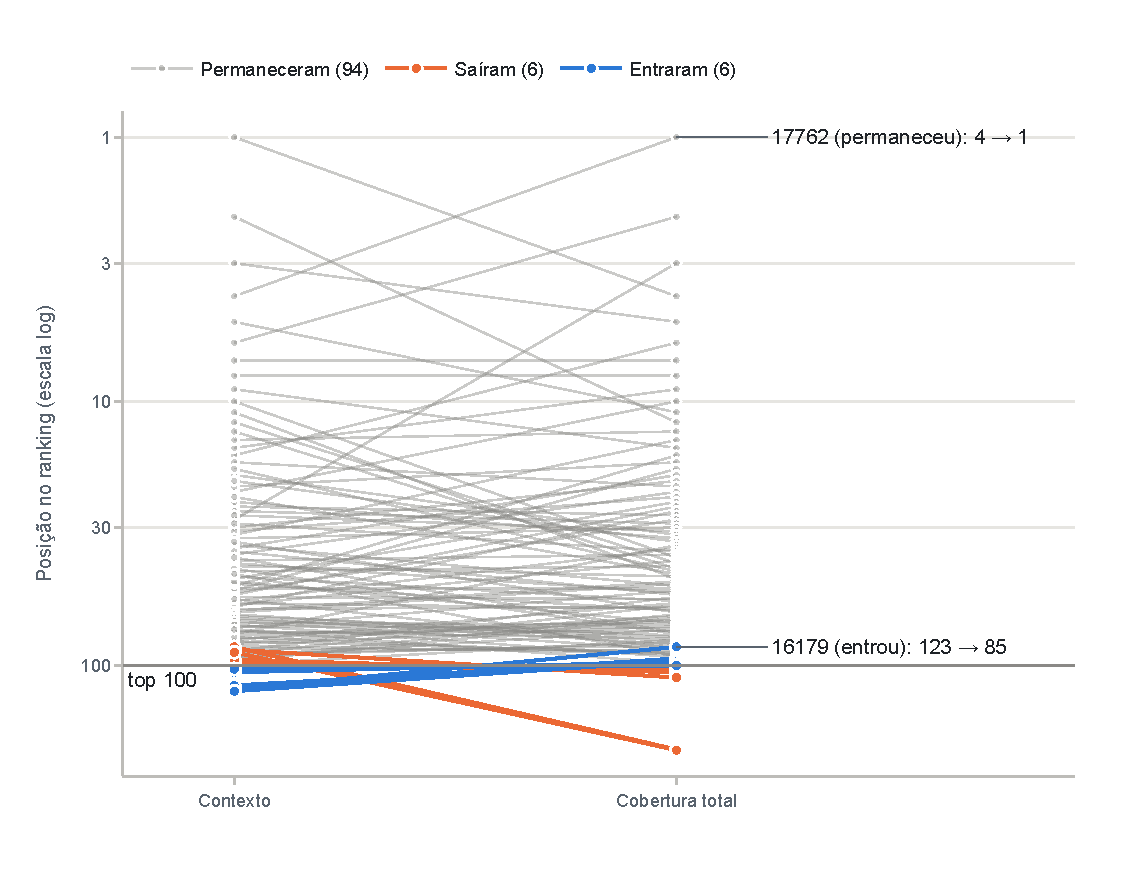
\includegraphics[width=\columnwidth]{G6_entradas_saidas_top100.pdf}
\caption{Top 100 do dia real com as ligações de contexto e com a cobertura total (GNN híbrida, seed 42). Cada linha liga as duas posições de uma carteira. Os casos da ficha T6 estão destacados.}
\label{fig:g6}
\end{figure}

\begin{figure*}[htbp]
\centering
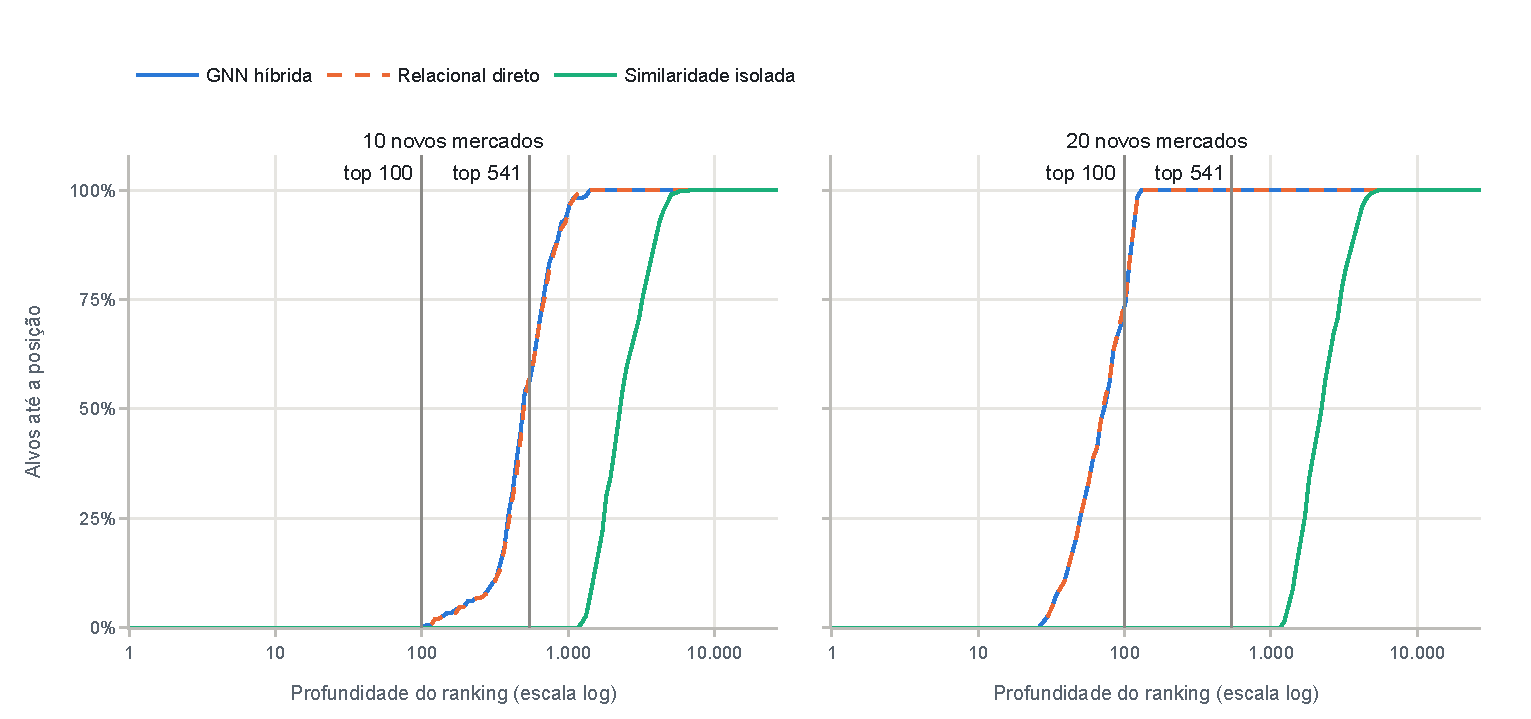
\includegraphics[width=\textwidth]{S1_recuperacao_acumulada.pdf}
\caption{Recuperação acumulada por profundidade do ranking no teste pareado: percentual dos 50 alvos até cada posição, média dos rankings (3 sorteios $\times$ 3 seeds; relacional tracejado, por sobrepor a GNN híbrida).}
\label{fig:s1}
\end{figure*}

\begin{figure}[htbp]
\centering
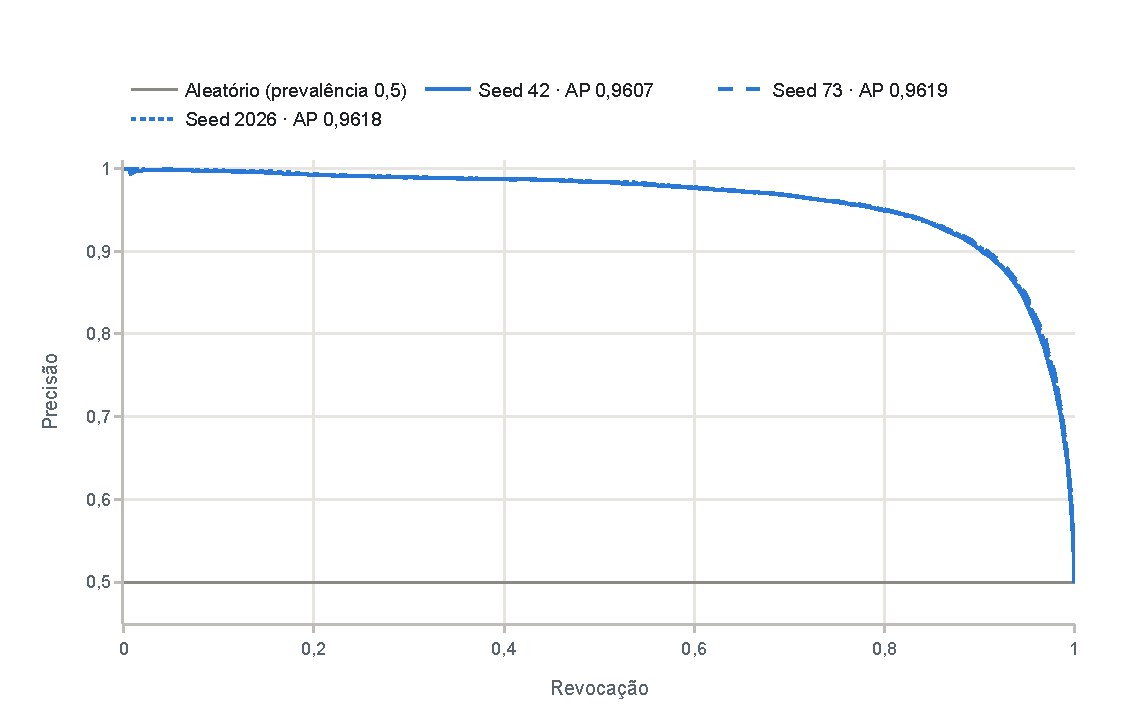
\includegraphics[width=\columnwidth]{S2_precisao_revocacao.pdf}
\caption{Curva precisão–revocação das ligações reservadas, por seed. Linha cinza: precisão de um classificador aleatório com negativos 1:1.}
\label{fig:s2}
\end{figure}

\begin{figure*}[htbp]
\centering
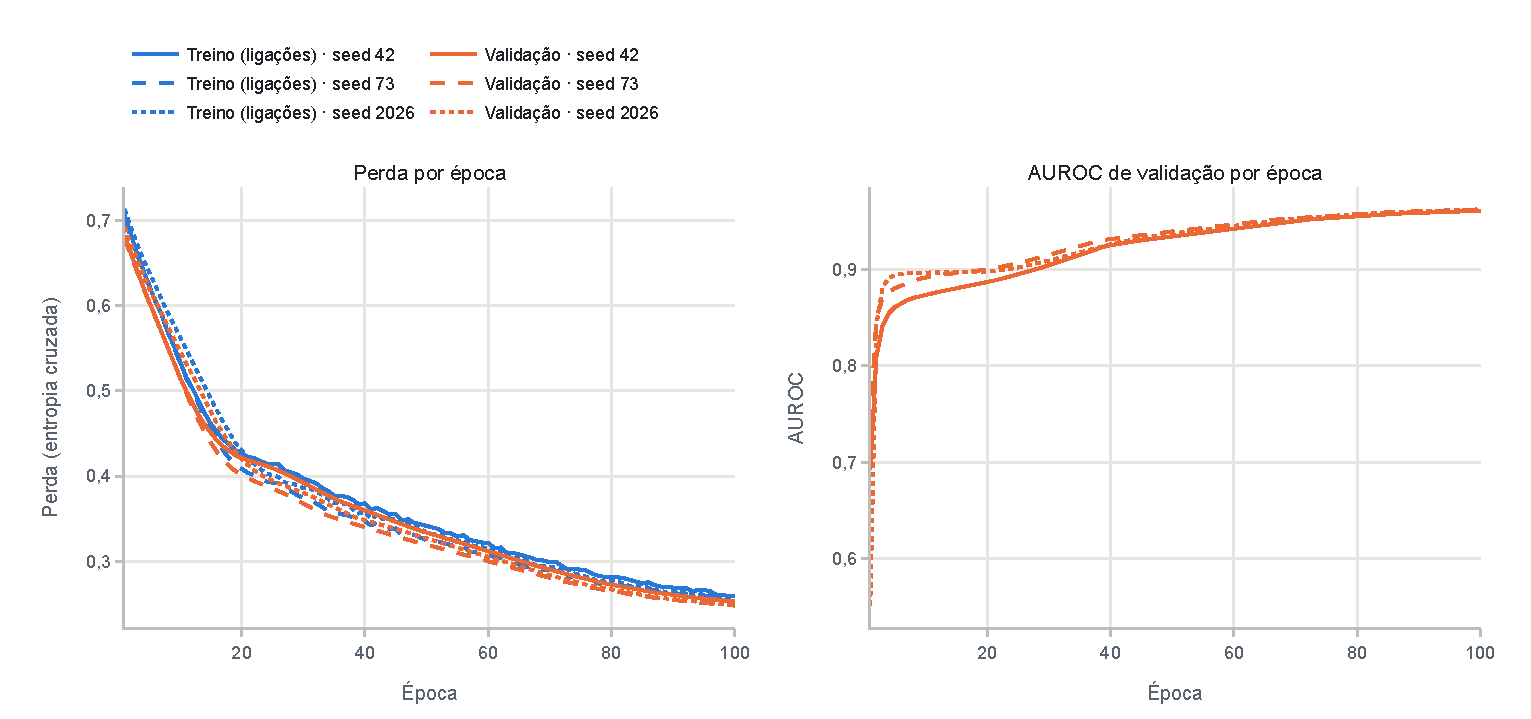
\includegraphics[width=\textwidth]{S3_perdas_treino.pdf}
\caption{Treino da GNN híbrida por seed (traço: 42 contínuo, 73 tracejado, 2026 pontilhado). A perda de treino inclui só o termo de ligações; o contraste (peso 0,1) fica de fora.}
\label{fig:s3}
\end{figure*}
